
\section{Sum of a Constant}

\section{Sum of a Finite Geometric Series}
The sum of the Geometric Series is most commonly stated as
\[ \sum_{i=0}^N{a^i} = \frac{1 - a^{N+1}}{1-a} \]

\subsection{Derivation}
\begin{align*}
\sum_{i=0}^N{a^i} &= a^0 + a^1 + a^2 + ... + a^N  \\
a\sum_{i=0}^N{a^i} &= a^1 + a^2 + ... + a^N + a^{N+1}
\end{align*}
Subtract the two equations
\begin{align*}
\sum_{i=0}^N{a^i} - a\sum_{i=0}^N{a^i} &= a^0 - a^{N+1}  \\
(1-a)\sum_{i=0}^N{a^i} &= 1 - a^{N+1} \\
\sum_{i=0}^N{a^i} &= \frac{1 - a^{N+1}}{1-a}
\end{align*}

\section{Sum of an Infinite Geometric Series}
The sum of the Geometric Series is most commonly stated as
\[ \sum_{i=0}^\infty{a^i} = \frac{1}{1-a} \]
if and only if \(a<1\)

\subsection{Derivation}
If we start with the summation of the finite Geometric Series, then take the limiting case where \(N\to \infty\) \\

\begin{align*}
\lim_{N\to \infty} \sum_{i=0}^N{a^i} = \frac{1 - a^{N+1}}{1-a} \\
\sum_{i=0}^\infty{a^i} = \frac{1 - \lim_{N\to \infty}a^{N+1}}{1-a}
\end{align*}
\\
\(\lim_{ N\to \infty}a^{N+1} =0 \) if and only if \(a<1\) \\
\begin{align*}
\sum_{i=0}^\infty{a^i} = \frac{1}{1-a}
\end{align*}
if and only if \(a<1\)


\section{$\sum\limits_{i=0}^N{i}$ : The Arithmatic Series}
The sum of the Arithmatic Series is most commonly stated as
\[\sum_{i=0}^N i= \sum_{i=1}^N i = \frac{N(N+1)}{2} \]

\subsection{Conjecture}
We can visualize adding 1 block to 2 blocks to 3 blocks and continue until we have N blocks.  As you can see, it sort of forms a triangle. \\
\begin{center}
\includegraphics[width=6cm]{Summations/sum_i_diag1}
\end{center}
What if we took the same triangle of blocks, flipped it upside down and joined it with the existing triangle?  It would form a rectangle of dimensions N x N+1. \\
\begin{center}
\includegraphics[width=8cm]{Summations/sum_i_diag2}
\end{center}
The area of this is \[A_{rectangle} = N(N+1)\] \\
\\
But what we want is the area of the tringle, just half of that \[A_{triangle}=\frac{N(N+1)}{2}\]
And this is \[ \sum_{i=0}^N i= \sum_{i=1}^N i = \frac{N(N+1)}{2}\]


\section{$\sum\limits_{i=0}^N{i^2}$}
The sum of \(i^2\) is most commonly stated as
\[\sum\limits_{i=0}^N{\frac{N(N+1)(2N+1)}{6}}\]

\subsection{Conjecture}
The same technique as used to demonstrate \(\sum\limits_{i=0}^N{i}\) can be used to demonstrate \(\sum\limits_{i=0}^N{i^2}\), except we have to use a 3-dimensional object.\\
\(\sum\limits_{i=0}^N{i^2}\) can be visualized in 3-dimensions as follows
\begin{center}
\includegraphics[width=8cm]{Summations/sum_i2_diag1}
\end{center}
Then a cube of dimensions N x (N+1) x (N+1) could be made.  See the diagram below\\
\begin{center}
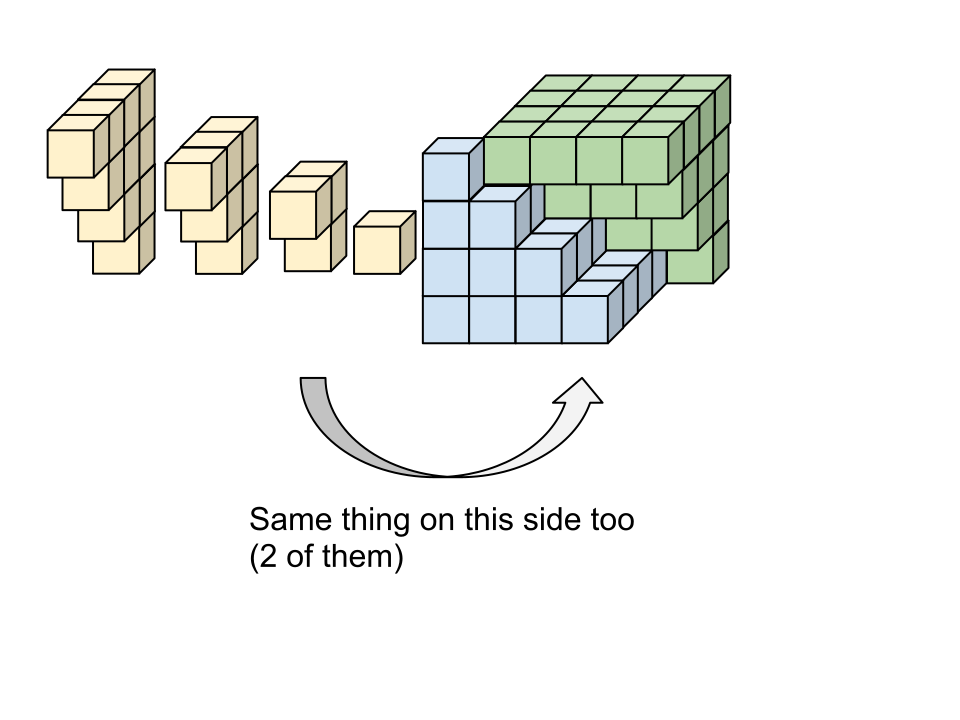
\includegraphics[width=8cm]{Summations/sum_i2_diag2}
\end{center}
The blue of the blue cubes is \(\sum\limits_{i=0}^N{i^2}\).  \\
The green of the blue cubes is \(\sum\limits_{i=0}^N{i^2}\).  \\
\\
The yellow cubes are \(\sum\limits_{i=0}^N{i}\), \(\sum\limits_{i=0}^{N-1}{i}\), \(\sum\limits_{i=0}^{N-2}{i}\), ...   \\
Or a more general way to write this would be \(\sum\limits_{i=0}^N{ \sum\limits_{j=0}^i{j}}\) \\
\\
\[ V_{prism} = N(N+1)^2 = 2\bigg(\sum\limits_{i=0}^N{i^2}\bigg) + 2\bigg(\sum\limits_{i=0}^N{ \sum\limits_{j=0}^i{j}} \bigg) \] \\
\begin{align*}
N(N+1)^2 =& 2\bigg(\sum\limits_{i=0}^N{i^2}\bigg) + 2\bigg(\sum\limits_{i=0}^N{ \frac{i(i+1)}{2}} \bigg) \\
N(N+1)^2 =& 2\sum\limits_{i=0}^N{i^2} + \sum\limits_{i=0}^N{ (i^2 + i)} \\
N(N+1)^2 =& 2\sum\limits_{i=0}^N{i^2} + \sum\limits_{i=0}^N{i^2 } + \sum\limits_{i=0}^N{i} \\
N(N+1)^2 =& 3\sum\limits_{i=0}^N{i^2} + \frac{N(N+1)}{2} \\
3\sum\limits_{i=0}^N{i^2} =& N(N+1)^2 - \frac{N(N+1)}{2} \\
3\sum\limits_{i=0}^N{i^2} =& \frac{3N(N+1)^2 - N(N+1)}{2} \\
\sum\limits_{i=0}^N{i^2} =& \frac{2N^3+3N^2+N}{6} \\
\end{align*}
And so
\[\sum\limits_{i=0}^N{i^2} = \frac{N(N+1)(2N+1)}{6}\] \\


\section{$\sum\limits_{i=0}^N{i^3}$ and beyond}
The sum of \(i^3\) is most commonly stated as
\[\sum\limits_{i=0}^N{i^3} = \bigg(\frac{N(N+1)}{2} \bigg)^2 = \bigg[\sum\limits_{i=0}^N{i^2} \bigg]^2\]

\subsection{Derivation}
The sum of \(i\) was derived by visualizing the stacking of 1-dimensional objects into a 2-dimensional shape.  Similarly, the sum of \(i^2\) was derived from stacking 2-dimensional objects into a 3-dimensional object. \\
\\
Unfortunately, our brains are not wired to visualize 4-dimensional objects, so we are left to derive the sum of \(i^3\) this with the abstraction of mathematics. \\
\\
The following is a mathematical technique that will be used to derive the sum of \(i^3\), however, the same technique may be used to the sum of \(i^p\)\\
\\
\(\sum\limits_{i=1}^N{i^4} = 1^4 + 2^4 + ... + N^4 \) \\
and \\
\(\sum\limits_{i=1}^N{(i+1)^4} = 2^4 + ... + N^4 + (N+1)^4\) \\
\\
These two sequences are equal if we take away the first term of the first summation and the last term of the second summation. \\
\begin{align*}
\bigg(\sum\limits_{i=1}^N{i^4} \bigg) - 1^4 = \bigg( \sum\limits_{i=1}^N{(i+1)^4} \bigg) -(N+1)^4 \\
\sum\limits_{i=1}^N{(i+1)^4} = \bigg(\sum\limits_{i=1}^N{i^4} \bigg) + (N+1)^4 - 1^4 \\
\sum\limits_{i=1}^N{(i^4 +4i^3 + 6i^2 + 4i +1)} = \bigg(\sum\limits_{i=1}^N{i^4} \bigg) + (N+1)^4 - 1^4 \\
\sum\limits_{i=1}^N{i^4} + 4\sum\limits_{i=1}^N{i^3} + 6\sum\limits_{i=1}^N{i^2} +4\sum\limits_{i=1}^N{i} + \sum\limits_{i=1}^N{1} = \bigg(\sum\limits_{i=1}^N{i^4} \bigg) + (N+1)^4 - 1^4 \\
4\sum\limits_{i=1}^N{i^3} = (N+1)^4 - 1^4  - 6\sum\limits_{i=1}^N{i^2} - 4\sum\limits_{i=1}^N{i} - \sum\limits_{i=1}^N{1} \\
 4\sum\limits_{i=1}^N{i^3} = (N+1)^4 - 1^4  - 6\bigg(\frac{(N(N+1)(2N+1)}{6}\bigg) - 4\bigg(\frac{N(N+1)}{2}\bigg) - N \\
4\sum\limits_{i=1}^N{i^3} = N^4 + 2N^3 + N^2\\
\sum\limits_{i=1}^N{i^3} = \frac{N^4}{4} + \frac{N^3}{2} + \frac{N^2}{4} = \bigg(\frac{N(N+1)}{2}\bigg)^2\\
\end{align*}
Notice that the limits of the above derivation were \( \sum\limits_{i=1}^N \), which was necessary for the derivation.  But in the end, adding a \(0^3\) does not change the summation, so
\[\sum\limits_{i=0}^N{i^3} = \bigg(\frac{N(N+1)}{2}\bigg)^2 = \bigg[ \sum\limits_{i=0}^N{i}\bigg]^2\]

